\chapter{Opis systemu}

Symulator robot�w jest doskona�ym narz�dziem dla ka�dej osoby zajmuj�cej si� robotyk�. Pozwala szybko przetestowa� r�ne algorytmy i konstrukcje oraz skomplikowane systemy realizuj�ce niecodzienne scenariusze. Jednym z takich narz�dzi jest darmowy program Gazebo, przeznaczony do tworzenia dok�adnych i efektywnych symulacji robot�w dzia�aj�cych w z�o�onych �rodowiskach. Posiada zaawansowany silnik fizyki, wysokiej jako�ci grafik� oraz wygodne i programowalne interfejsy.
\\ \\
To powy�ej to pr�ba t�umaczenia opisu poni�ej ze strony Gazebo :D
\\ \\
Robot simulation is an essential tool in every roboticist's toolbox. A well-designed simulator makes it possible to rapidly test algorithms, design robots, perform regression testing, and train AI system using realistic scenarios. Gazebo offers the ability to accurately and efficiently simulate populations of robots in complex indoor and outdoor environments. At your fingertips is a robust physics engine, high-quality graphics, and convenient programmatic and graphical interfaces. Best of all, Gazebo is free with a vibrant community.

\section{Okienka}
Funkcjonalno�ci + Implementacja
\subsection{Konfiguracja �wiata}
\begin{figure}[htbp]
 \centering
 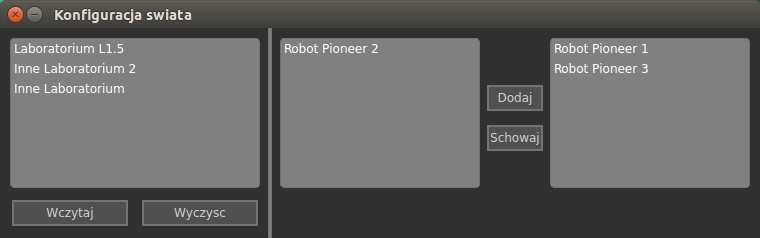
\includegraphics[width=1.0\textwidth]{opis_systemu/materialy/konfiguracja_swiata.jpeg}
 \label{fig:konfiguracja_swiata}
 \caption{Okno konfiguracji �wiata}
\end{figure}

Okno konfiguracji �wiata pozwala zmodyfikowa� zawarto�� sceny. Domy�lnie �adowany jest jedynie ground plane, czyli bazowe pod�o�e, na kt�rym umieszczane s� modele. Okno umo�liwia szybkie rozpocz�cie pracy z wybranymi modelami. U�ytkownik ma mo�liwo�� wyboru sali z listy dost�pnej w lewej cz�ci okna. Lista tworzona jest na podstawie plik�w konfiguracji sali z rozszerzeniem .txt znajduj�cych si� w folderze worlds, w katalogu �r�d�owym Gazebo. Przyk�adowy zestaw danych ma nast�puj�c� posta�:
\begin{lstlisting}[language=bash]
smietnik 4.6 1.3 0 0 0 0
szafa 1.5 -3.6 0 0 0 0
kaloryfer -4.5 1.6 0 0 0 1.570796
kaloryfer -4.5 -2.8 0 0 0 1.570796
stol -2.4 2.5 0 0 0 0
stol -4 2.5 0 0 0 0
stol -0.7 -3.4 0 0 0 0
krzeslo -1.7 -2.6 0 0 0 0
krzeslo -1 -2.6 0 0 0 0
krzeslo -0.1 -2.6 0 0 0 0
\end{lstlisting}
W ka�dej linii dodawany jest jeden z dost�pnych modeli. Trzy pierwsze liczby oznaczaj� pozycj� modelu na scenie (X, Y, Z). Pozosta�e okre�laj� orientacj� wok� ka�dej z osi.

Naci�niecie przycisku "Wczytaj" powoduje wyczyszczenie sceny i za�adowanie wybranej sali. Przycisk "Wyczy��" usuwa wszystkie statyczne modele.

Prawa strona okna konfiguracji �wiata pozwala wybra� liczb� robot�w Pioneer, z kt�rymi u�ytkownik chce rozpocz�� prac�. Liczba pozycji w lewym polu okre�la ile robot�w jest dost�pnych, natomiast liczba pozycji w prawym polu definiuje liczb� robot�w na scenie. Zawarto�� p�l mo�na modyfikowa� za pomoc� przycisk�w "Dodaj" i "Schowaj".
% Krzysztof Kwieci�ski
\subsection{Zarz�dzanie robotami}
Okienko \texttt{Zarz�dzanie robotami} umo�liwia ustawianie pozycji oraz orientacji wybranego robota na scenie.

Zak�adki umo�liwiaj� wyb�r \texttt{Pioneera}, kt�rego pozycj� chcemy zmieni�. Aktywne s� tylko zak�adki skojarzone z~robotami dodanymi aktualnie do �wiata. 

Po wyborze zak�adki mo�liwe jest podanie nowych wsp�rz�dnych $XY$ oraz orientacji $\theta$ robota. W~polach odpowiedzialnych za pozycj� i~orientacj� kolor informuje o~poprawno�ci wprowadzonych danych -- zielony oznacza poprawnie wype�nione pola, natomiast czerwony b��dnie. 

Przyci�ni�cie przycisku \texttt{Ustaw} powoduje ustawienie \texttt{Pioneera} zgodnie z~��daniem. Przycisk \texttt{Reset} przenosi robota do punktu $(0, 0)$ i~ustawia jego orientacj� na~$0$. 

Po zmianie zak�adki lub ustawieniu/zresetowaniu pozycji, w~polach wy�wietlane s� aktualne wsp�rz�dne robota.

\begin{figure}[htbp]
 \centering
 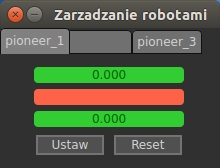
\includegraphics[]{opis_systemu/materialy/zarzadzanie_robotami.jpeg}
 \label{fig:zarzadzanie_robotami}
 \caption{Okno zarz�dzania robotami}
\end{figure}

\subsubsection{Implementacja}
Klasa odpowiadaj�ca za ca�e okienko to \texttt{RobotManagementWindow}. Dziedziczy ona po klasie \texttt{QDialog}. 

Sloty odpowiadaj�ce za to co dzieje si� w~oknie w~momencie dodania lub schowania robota to:
\begin{lstlisting}[language=C++, numbers=none]
public slots:
	void onAddRobot(int id);
	void onHideRobot(int id);
\end{lstlisting}
W~momencie otrzymania odpowiednich sygna��w aktywowana b�d� dezaktywowana jest stosowna zak�adka, a~tak�e ustawiane s� warto�ci w~polach.

Wy�wietlanie pozycji i~orientacji robota mo�liwe jest dzi�ki subskrybowaniu odpowiedniego tematu i~wywo�aniu funkcji aktualizuj�cej pozycj� robota:
\begin{lstlisting}[language=C++, numbers=none]
this->sub = node->Subscribe("~/pose/info", 
                            &RobotManagementWindow::OnPoseMsg, this);
\end{lstlisting}

Klasa odpowiadaj�ca za wygl�d  pojedynczej zak�adki oraz g��wn� funkcjonalno�� okienka to \texttt{RobotManagementTab}. Dziedziczy ona po klasie \texttt{QWidget}. Jej kluczowe metody to:
\begin{lstlisting}[language=C++, numbers=none]
private slots:
	void on_pushButtonUstaw_clicked();
	void on_pushButtonReset_clicked();
\end{lstlisting}
Odpowiadaj� one za ustawienie b�d� zresetowanie pozycji robota. Przyci�ni�cie kt�rego� z~przycisk�w skutkuje wywo�aniem us�ugi \texttt{/gazebo/set\_model\_state}.














\subsection{Wyniki symulacji}

\subsubsection{Funkcjonalno��}

Okno wykres�w oferuje w pierwszej zak�adce podgl�d na pozycj� X-Y wszystkich robot�w dost�pnych na scenie. 

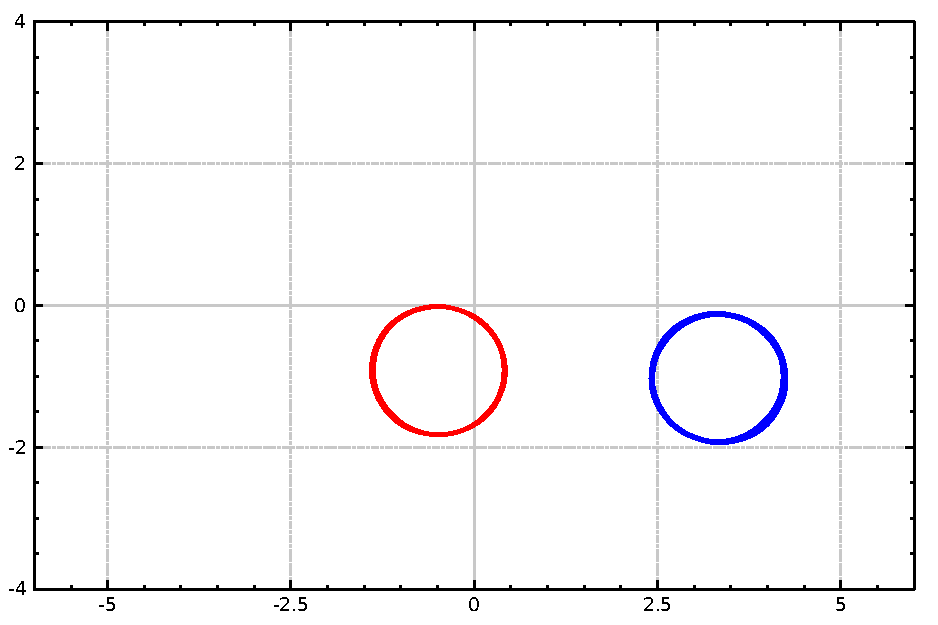
\includegraphics[height=5cm]{opis_systemu/wyniki_symulacji/images/robot_trace.pdf}

Na kolejnych wykresach ilustrowana jest pozycj� robota w osiach X,Y oraz orientacje wzgl�dem czasu symulacji.

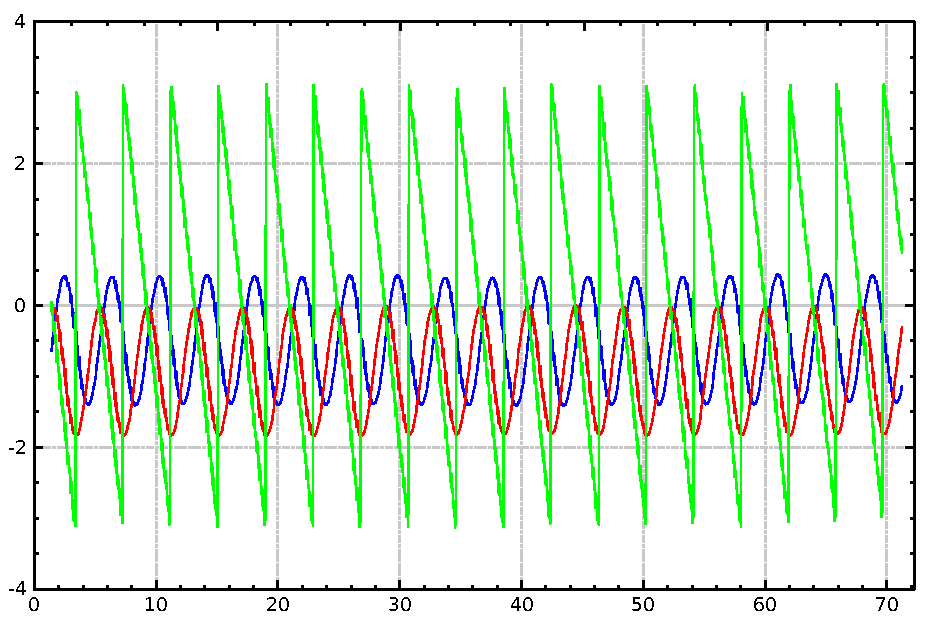
\includegraphics[height=5cm]{opis_systemu/wyniki_symulacji/images/robot_pose_2.pdf}

Okno zawiera dwa przyciski pozwalaj�ce na zresetowanie danych o robotach (czas symulacji nie zostaje zresetowany). Oraz przycisk pozwalaj�cy na zapis danych.

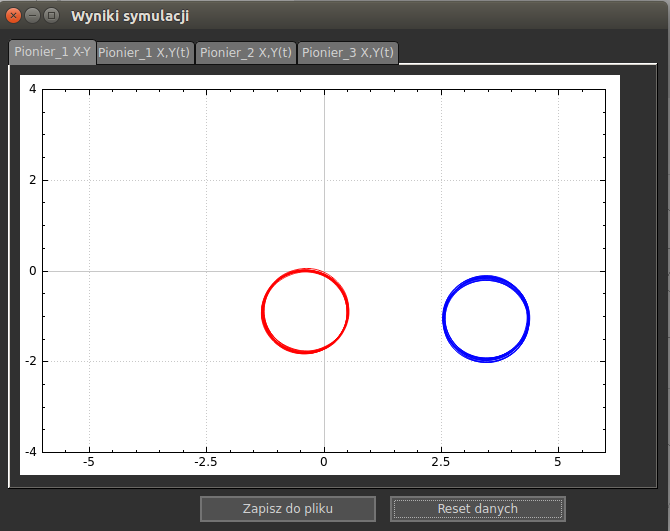
\includegraphics[height=5cm]{opis_systemu/wyniki_symulacji/images/zrzut_2.png}

Dane znajduj� si� w katalogu g��wnym kontenera. Wykresy s� zapisywane w postaci plik�w pdf. Program generuje r�wnie� plik csv z danymi uzyskanymi podczas symulacji. \\ \#Pionier1 X,Pionier1 Y,Pionier1 W,Pionier2 X,Pionier2 Y,Pionier2 W,Pionier3 X,Pionier3 Y,Pionier3 W,time\\
2.4122,-1.15,1.6118,-0.63934,-0.040688,0.047668,0,1,1,1.389\\
2.4082,-1.1215,1.5783,-0.61012,-0.036784,0.01829,0,0,0,1.409\\
2.4072,-1.1129,1.5685,-0.60134,-0.035781,0.0094779,0,0,0,1.415
\subsubsection{Implementacja}

Do stworzenia wykres�w wykorzystano biblioteki QT i QCustomPlot. Dane o pozycji robot�w pionier, pobierane s� w klasie world\_plugin z topic-�w Gazebo. Komunikacj� mi�dzy oknami zapewniono wykorzystuj�c biblioteki gazebo z funkcjami subscriber i publisher. Dane o pozycji robot�w przesy�ane s� do klasy ResultWindow odpowiedzialnej za rejestrowanie, wy�wietlanie i zapisywanie informacji o robotach.
\section{Pluginy}
Plugin, czyli wtyczka, jest cz�ci� kodu, kt�ry zosta� skompilowany jako wsp�dzielona biblioteka i dodany do symulatora. Ma on dost�p do wszystkich funkcjonalno�ci Gazebo poprzez gotowe klasy j�zyka C++. Pluginy s� bardzo przydatne nie tylko ze wzgl�du na mo�liwo�� kontroli dowolnych modu��w symulatora, ale r�wnie� ze wzgl�du na swoj� elastyczno��. Z �atwo�ci� mo�na je dodawa� i usuwa� z systemu. W Gazebo jest dost�pnych 6 typ�w wtyczek:
\begin{itemize}
\item World
\item Model
\item Sensor
\item System
\item Visual
\item GUI
\end{itemize}
Oprogramowanie utworzone w ramach projektu wykorzystuje dwie z nich: GUI i World.
\subsection{GUI}
Plugin GUI jest bezpo�rednio zwi�zany z graficznym interfejsem u�ytkownika. Z jego poziomu mo�na w prosty spos�b dodawa� elementy takie jak przyciski, okna, listy czy pola tekstowe. Wtyczka dodawana jest do pliku konfiguracji �wiata w nast�puj�cy spos�b:
\begin{lstlisting}[language=bash]
...
<gui fullscreen='0'>
<plugin name='SimulationGUI' filename='lib_simulation_gui_plugin.so'/>
...
\end{lstlisting}
Z wykorzystaniem pluginu GUI i bibliotek Qt utworzona zosta�a w g�rnej cz�ci okna symulacji belka z trzema przyciskami otwieraj�cymi opisane wcze�niej okna konfiguracyjne, zwi�kszaj�ce funkcjonalno�� symulatora.

Wtyczka interfejsu ma ograniczony dost�p do zasob�w Gazebo. Chc�c z jej pomoc� dokonywa� modyfikacji na scenie konieczne jest wysy�anie odpowiednich komend do pluginu World. W tym celu w projekcie wykorzystano komunikacj� za pomoc� temat�w symulatora. Wtyczka GUI pe�ni rol� nadawcy (publisher), natomiast wtyczka World jest subskrybentem (subscriber). Wiadomo�ci mog� mie� dowolny, wcze�niej zdefiniowany format. Przyk�adowo, je�eli wysy�ane s� informacje o pozycji robota, format wiadomo�ci zawiera nazw� modelu i sze�� zmiennych liczbowych przechowuj�cych pozycj� i orientacj�.

Tworzenie temat�w i konfiguracja komunikacji realizowana jest z poziomu kodu, z~wykorzystaniem bibliotek Gazebo.

\subsection{World}
World plugin pozwala na edycj� r�nych parametr�w �wiata, przyk�adowo silnika fizyki lub o�wietlenia. Ponadto umo�liwia modyfikowanie sceny i znajduj�cych si� na niej obiekt�w. Wtyczka jest bezpo�rednio zwi�zana z plikiem ustawie� z rozszerzeniem .world, �adowanym podczas uruchamiania Gazebo. Ten plik jest r�wnie� odpowiedzialny za uruchomienie wybranej wtyczki:
\begin{lstlisting}[language=bash]
<sdf version='1.6'>
<world name='default'>
<plugin name='projekt_przejsciowy' filename='libprojekt_przejsciowy.so'/>
...
\end{lstlisting}
Budowa pluginu World w pliku �r�d�owym jest do�� prosta i intuicyjna. Minimalny kod pozwalaj�cy skompilowa� bibliotek� ma nast�puj�c� posta�:
\begin{lstlisting}[language=bash]
#include <gazebo/gazebo.hh>

namespace gazebo
{
  class WorldPluginTutorial : public WorldPlugin
  {
    public: WorldPluginTutorial() : WorldPlugin()
    {
      printf("Witaj!\n");
    }
    public: void Load(physics::WorldPtr _world, sdf::ElementPtr _sdf)
    {
    }
  };
  GZ_REGISTER_WORLD_PLUGIN(WorldPluginTutorial)
}
\end{lstlisting}
Na podstawie powy�szego kodu, przy odpowiedniej konfiguracji plik�w makefile mo�na zbudowa� plik z rozszerzeniem .so, kt�ry jako biblioteka jest dodawany do programu.
\section{Integracja Gazebo z ROS}
G��boka integracja Gazebo z ROS jest najwi�ksz� zalet� tego symulatora. Umo�liwia j� zestaw dostarczanych plugin�w do ROS w pakiecie gazebo\_ros\_pkgs.
Podstawowe funkcjonalno�ci dostarczane razem z pakietem:
\begin{itemize}
\item pomimo integracji Gazebo pozostaje nadal samodzielnym systemem,
\item mo�liwo�� zbudowania pakiet�w Gazebo w catkin,
\item zmniejszenie ilo�ci kodu potrzebnego do symulacji,
\item udost�pnia u�ytkownikowi szereg us�ug i temat�w ROS do zarz�dzania symulacj� (wymienione na Rysunku \ref{fig:ros_integracja})
\end{itemize}

\begin{figure}[htbp]
 \begin{center}
  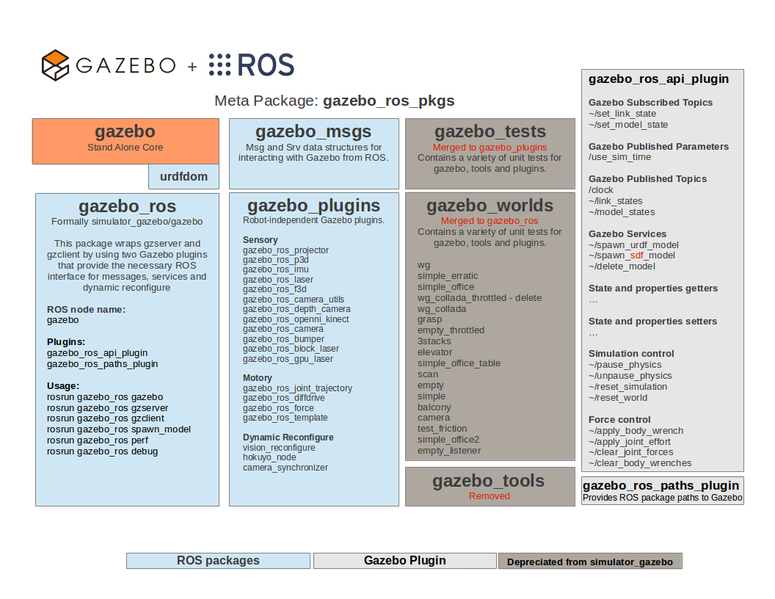
\includegraphics[width=\textwidth]{opis_systemu/materialy/gazeborosapi}   
  \caption{Schemat prezentuj�cy funkcje udost�pniane przez gazebo\_ros\_pkgs}
  \label{fig:ros_integracja}
 \end{center}
\end{figure} 

\subsection{Kompilacja pakiet�w Gazebo przy u�yciu catkin}
Jak zaznaczono wcze�niej, mo�liwe jest bezpo�rednie u�ycie systemu catkin do budowania pakiet�w napisanych dla Gazebo. Wymaga�o to stworzenia catkin workspace -- katalogu, w kt�rym budowane s� pakiety catkin. Stworzone przez nas pluginy Gazebo zosta�y zebrane i tak skonfigurowane, �e tworz� pakiet kompatybilny z ROS.

Po uruchomieniu, Gazebo tworzy w�asny w�ze� do komunikacji z ROS. Dzi�ki kompilacji poprzez catkin, pluginy Gazebo maj� dost�p do ROSa, bezpo�rednio w kodzie mo�emy odwo�ywa� do jego funkcji. Aby si� o tym upewni�, w World plugin umieszczono poni�szy kod, kt�ry zatrzymuje dzia�anie Gazebo w przypadku braku komunikacji z ROS.

\begin{lstlisting}[language=c]
...                                                                                   
if ( !ros::isInitialized() )
{
	ROS_FATAL_STREAM("A ROS node for Gazebo has not been initialized");
	return;
}
...
\end{lstlisting}

\subsection{Uruchamianie Gazebo przy u�yciu narz�dzi z ROS}
Dzi�ki u�yciu catkin'a mo�emy uruchamia� Gazebo za pomoc� narz�dzia roslaunch, kt�re pozwala na automatyczne wywo�ywanie w�z��w ROS oraz wst�pn� konfiguracj�. U�atwia to start skonfigurowanego do pracy �rodowiska, co sprowadza si� do jednego polecenia:
\begin{verbatim}
$ roslaunch projekt_przejsciowy l15.launch
\end{verbatim}
Aby to umo�liwi�, przygotowano odpowiedni plik l15.launch w podkatalogu stworzonego pakietu Gazebo $launch$. Plik launch mo�e przy uruchomieniu wczytywa� plik world z~konfiguracj� Gazebo lub umieszcza� modele w odpowiednich miejscach.

\subsection{Udost�pnione funkcjonalno�ci do komunikacji ROS}
Jak wida� na Rysunku \ref{fig:ros_integracja}, Gazebo udost�pnia szereg funkcjonalno�ci kt�rych mo�na u�y� do integracji z ROS. 

Dla projektu najwi�ksze znaczenie mia�y pluginy wysy�aj�ce dane z czujnik�w na robocie, takich jak skaner laserowy czy kamera oraz umo�liwiaj�ce sterowanie nap�dem robota. Zosta�y one zintegrowane z modelem Pioneera.

W�ze� tworzony przez Gazebo publikuje informacje na zewn�trz za pomoc� temat�w, np. \~/model\_states, wysy�aj�cy informacje o stanie modeli aktualnie u�ywanych w symulacji. W�ze� dostarcza r�wnie� us�ugi ROS'a, takie jak \~/spawn\_urdf\_model do �adowania modeli robot�w w formacie URDF, czy \~/delete\_model do usuwania modeli. Mog� zosta� one wykorzystane przez u�ytkownika naszego systemu do kontroli symulacji i zbierania danych symulacyjnych.
\section{Modele}

Modele u�yte do stworzenia laboratorium L1.5 zosta�y wykonane w programach Inventor Professional oraz Blender.

Elementy wyposa�enia wn�trza takie jak sto�y, krzes�a, grzejniki, szafa oraz �mietnik zaprojektowane zosta�y w Inventorze, natomiast sama sala (�ciany) w programie Blender. Wszystkie stworzone elementy opracowane zosta�y w oparciu o pomiary rzeczywistych mebli, przedmiot�w i �cian w sali L1.5 w budynku C-16. Nast�pnie wszystkie elementy zosta�y przekonwertowane przy u�yciu programu Blender do formatu Collada (.dae), aby mo�liwe by�o wykorzystanie ich w Gazebo.

Modele zosta�y r�wnie� posk�adane w Blenderze w celu wyrenderowania widok�w z r�nych miejsc sali:

\begin{center}

	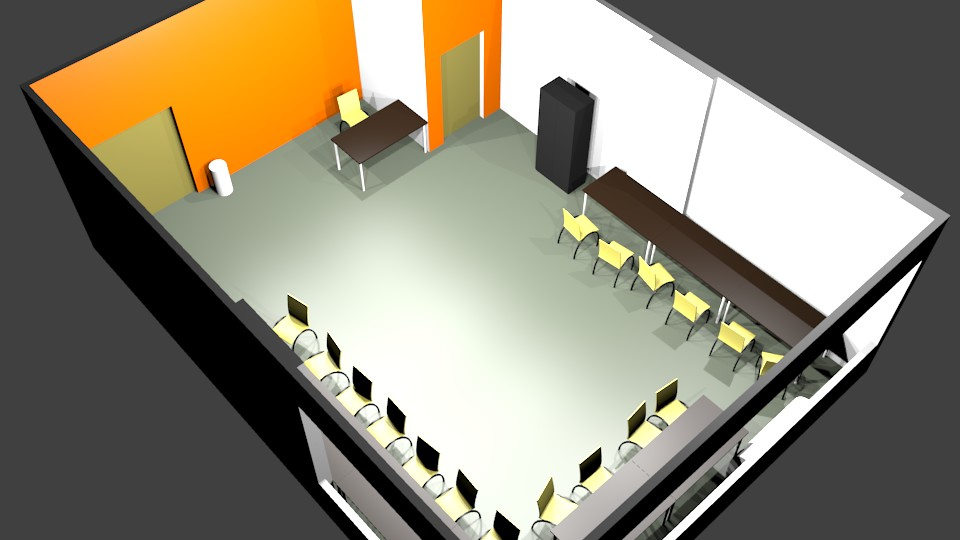
\includegraphics[width=12cm]{opis_systemu/materialy/R4.jpg}
	
	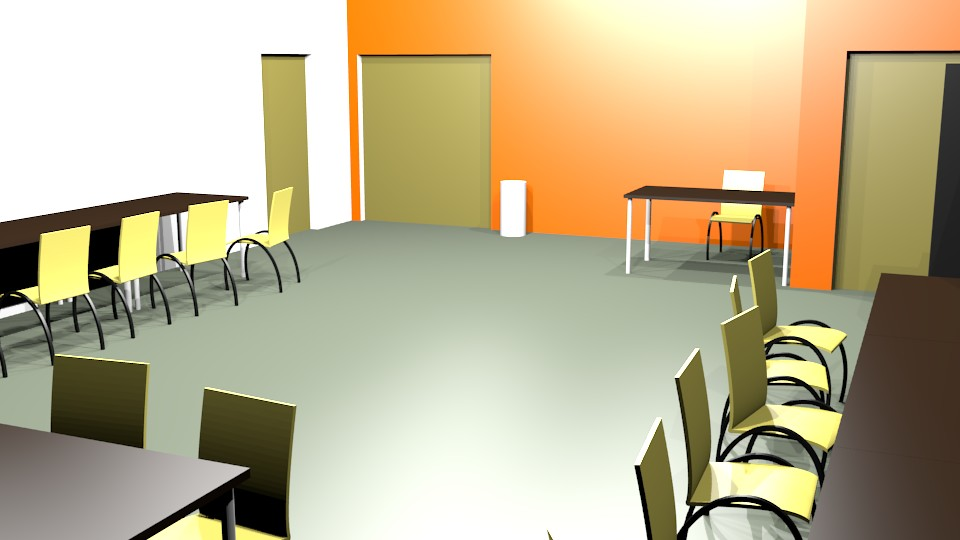
\includegraphics[width=12cm]{opis_systemu/materialy/R1.jpg}

\end{center}

Aby stworzone modele mog�y by� u�yte w Gazebo, konieczne by�o jeszcze napisanie plik�w konfiguracyjnych "model.config" oraz "model.sdf".
\\
Plik "model.config" zawiera takie informacje jak:
\begin{itemize}
\item nazwa obiektu
\item lista wersji pliku .sdf
\item informacje o autorze
\end{itemize}
W pliku "model.sdf" przechowywane s� informacje na temat:
\begin{itemize}
\item w�a�ciwo�ci fizycznych obiektu (masa, momenty bezw�adno�ci)
\item statyczno�ci obiektu (mo�liwo�ci poruszenia przez inny obiekt)
\item geometrii obiektu wyko�ystywanej przy kolizji z innymi obiektami
\item wizualizacji obiektu w symulacji
\end{itemize}
W przypadku modeli z�o�onych, takich jak np. roboty, plik "model.sdf" mo�e zawiera� r�wnie�:
\begin{itemize}
\item informacje o w�a�ciwo�ciach fizycznych poszczeg�lnych cz�on�w obiektu
\item parametry po��cze� kinematycznych mi�dzy cz�onami
\item pluginy wyko�ystywane w modelu
\item dane o czujnikach i ich umieszczeniu
\end{itemize}
Do stworzenia modelu robota Pioneer wykorzystano pliki zawarte w Gazebo, jednak aby mo�na by�o go u�y� w symulacjach konieczne by�o zaimplementowanie jego funkcjonalno�ci w pliku .sdf. W tym celu dodano pluginy do obs�ugi nap�d�w oraz sensor�w, kt�re zosta�y dodane do modelu.

Dzi�ki tym zabiegom podczas dodawania robota w symulacji tworzone s� tematy pozwalaj�ce na komunikacj� z modelem robota.